\section{Experiments and Results}
\subsection{Experimental Setup}
The proposed framework was deployed on a real robotic baggage-handling platform, shown in Fig.~\ref{fig:setup}. The platform consists of a collaborative robotic arm equipped with a hybrid suction--gripper end-effector, a conveyor belt operating at 493~mm/s, and an Orbbec Gemini 435Le RGB-D camera with a resolution of $640\times400$ at 20~FPS. All algorithms were executed on an embedded AX650N processor. MSAM-Net inference, PX3C filtering, and CAOS stabilization were executed at every frame. DKF state prediction was executed every five frames, corresponding to approximately 200$\mathrm{ms}$ and a conveyor displacement of about 98.6~mm.

\begin{figure}[!t]
\centering
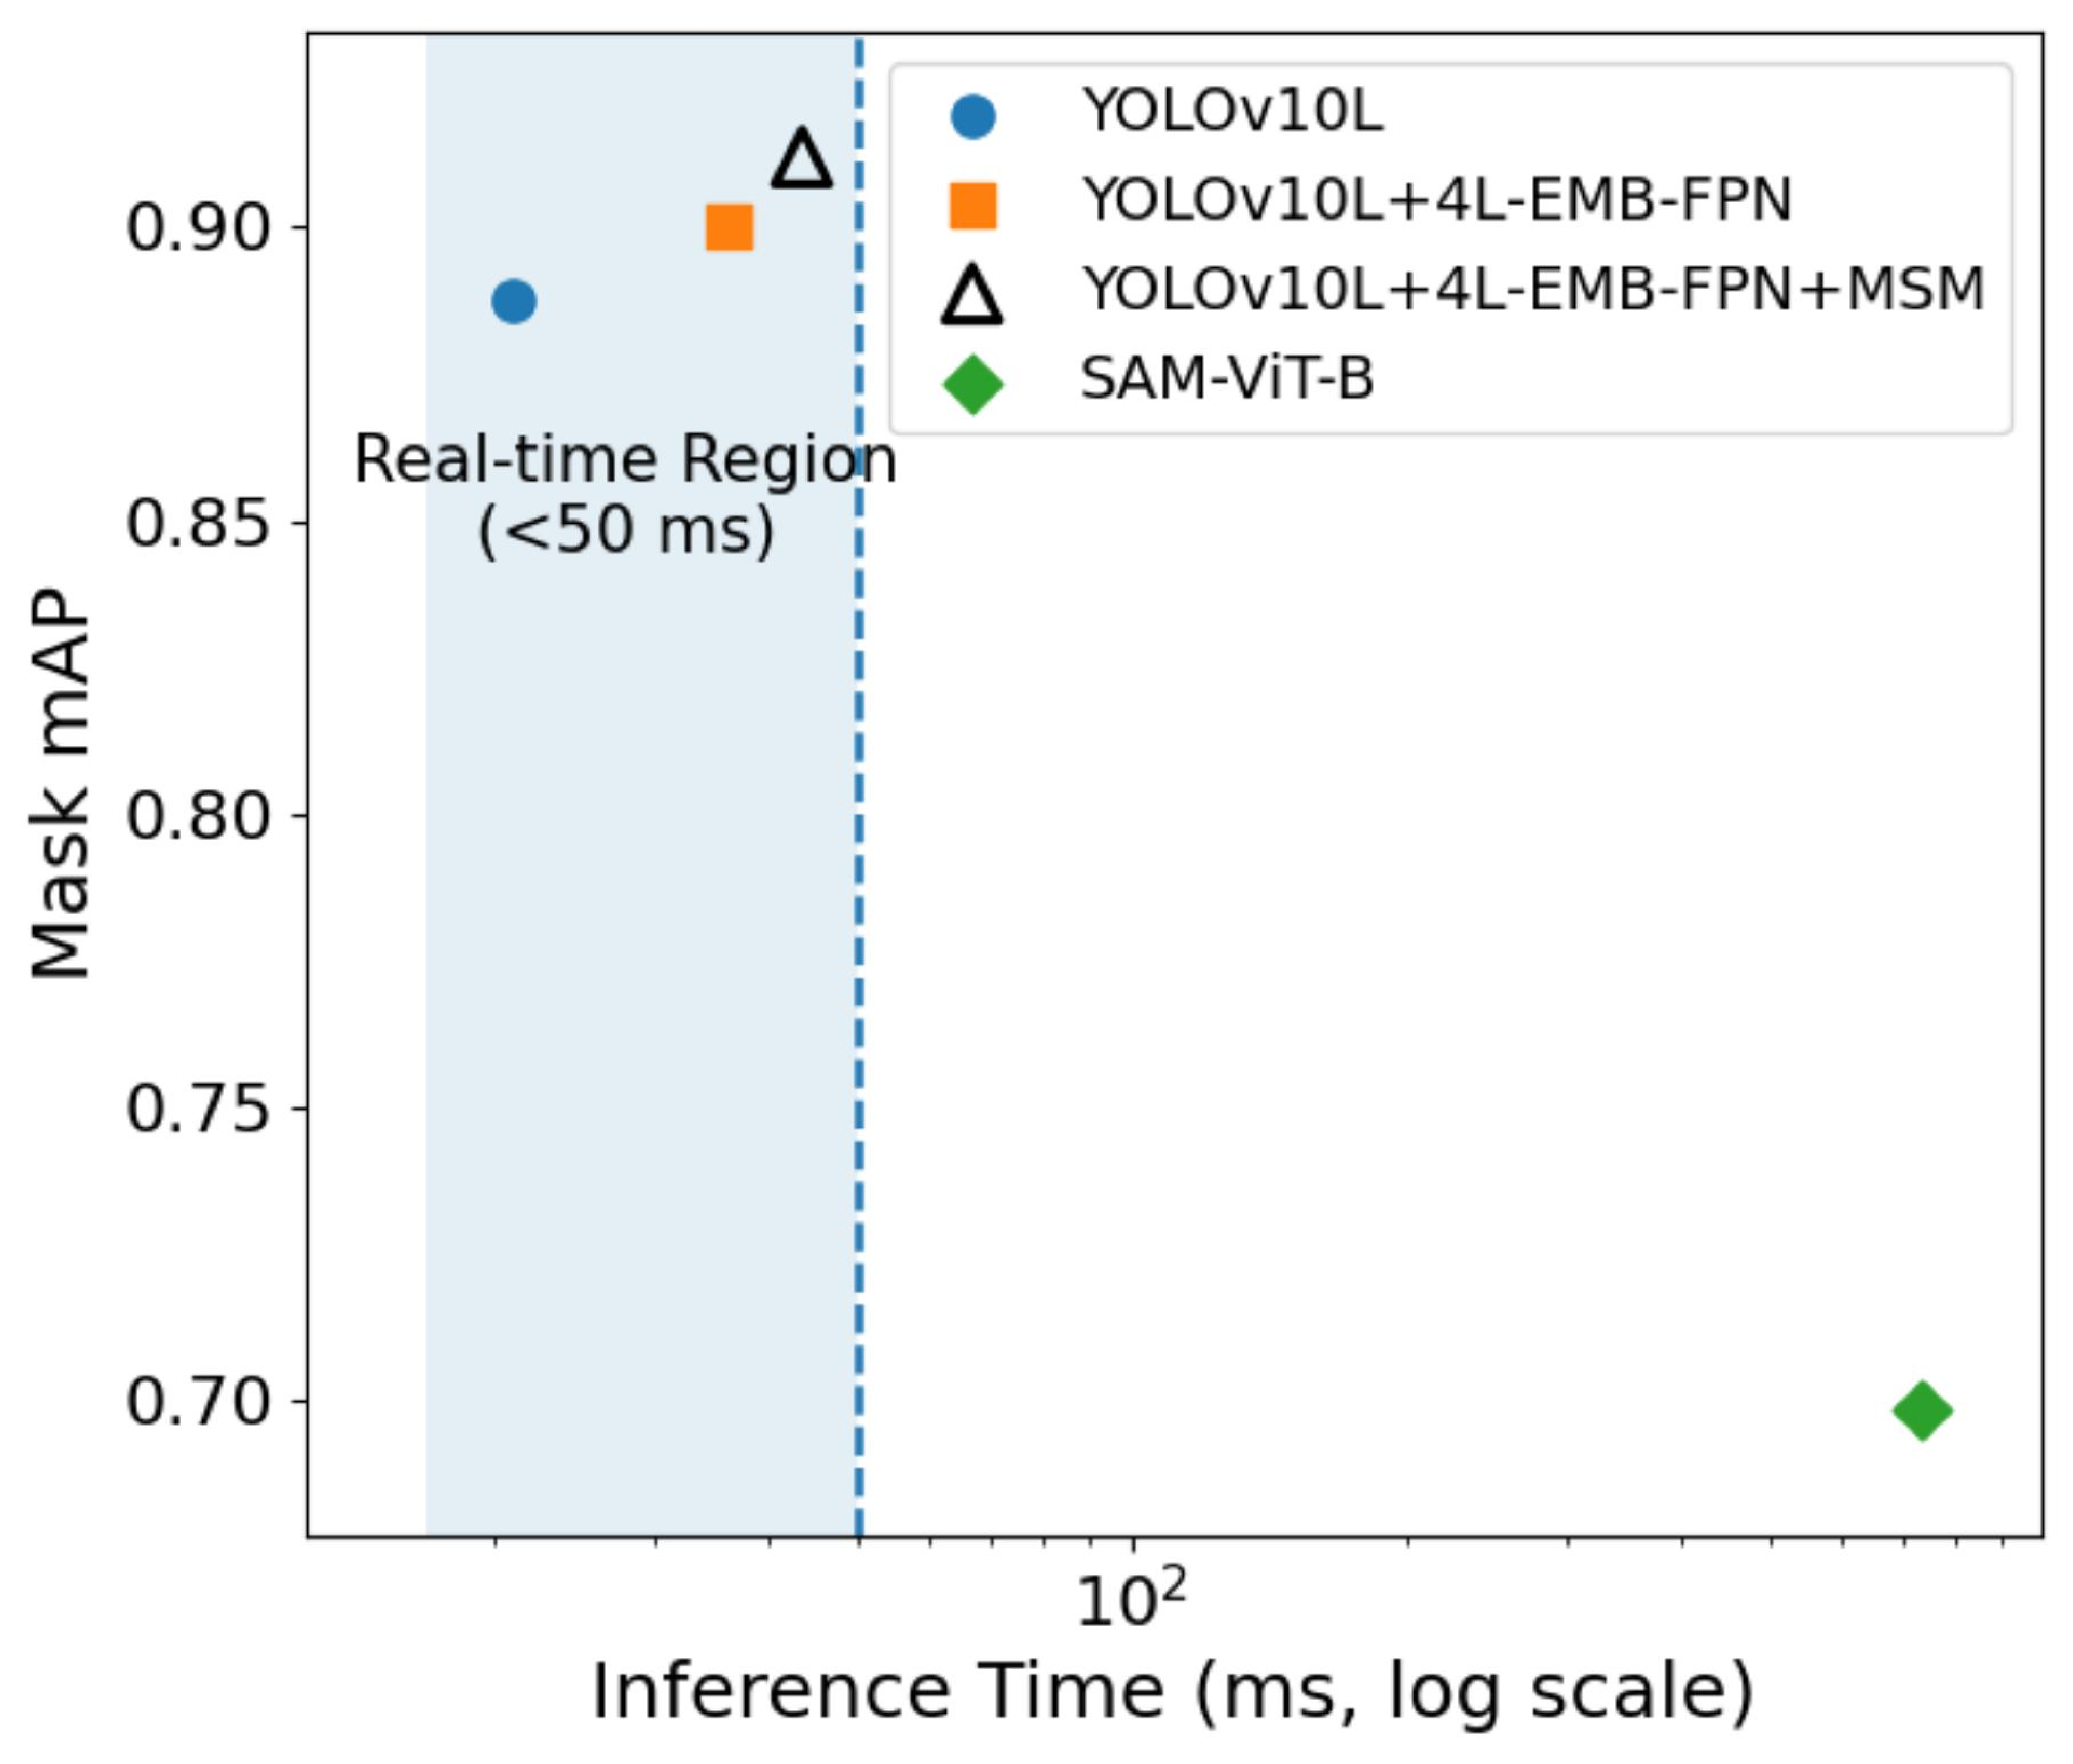
\includegraphics[width=\columnwidth]{figures/fig6.pdf}
\caption{Mask mAP versus inference time for different segmentation models.}
\label{fig:comparison_time}
\end{figure}

The baggage distribution was designed according to airport statistics collected from three airports across eight flights, including 515 items. Suitcases accounted for 94\% of the samples, soft bags for 5\%, and irregular objects for 1\%. More than 90\% of the samples contained strong tag interference. To simulate operational difficulty, random scenarios were generated, including single baggage placement (83\%), two-item contact (10\%), three-item stacking (2\%), and sidewall occlusion (5\%).

For 2D segmentation evaluation, a dataset named SegData was constructed with 49,359 training images and 10,344 testing images captured under different illumination, viewpoints, and distances. For 3D modeling evaluation, OBBData-test was constructed from 1,209 suitcase samples selected from SegData-test. The ground-truth OBBs were manually refined in 3D point clouds. Suitcases were selected because they dominate the baggage distribution and provide stable centroid and yaw references, whereas soft bags are deformable and difficult to annotate consistently.

\subsection{Segmentation Performance}
Three models were trained on SegData-train and evaluated on SegData-test: YOLOv10L, YOLOv10L with 4L-EMB-FPN, and YOLOv10L with both 4L-EMB-FPN and MSM, i.e., MSAM-Net. Table~\ref{tab:seg} reports the quantitative segmentation results.

\begin{table}[!t]
\centering
\caption{Segmentation performance on SegData-test.}
\label{tab:seg}
\begin{tabular}{lcc}
\toprule
Method & Box mAP & Mask mAP \\
\midrule
YOLOv10L & 0.9185 & 0.8877 \\
+ 4L-EMB-FPN & 0.9417 & 0.9004 \\
+ MSM (MSAM-Net) & 0.9524 & 0.9120 \\
\bottomrule
\end{tabular}
\end{table}

The 4L-EMB-FPN improves mask mAP by 1.27\% compared with the YOLOv10L baseline, and the full MSAM-Net further increases the gain to 2.43\%. These results show that enhanced multi-scale aggregation and attention-guided mask refinement improve segmentation quality under tag and strap interference.

Inference latency on the AX650N processor is reported in Table~\ref{tab:latency}. MSAM-Net increases the inference time from 21.1$\mathrm{ms}$ to 43.6$\mathrm{ms}$, but remains below the 50$\mathrm{ms}$ real-time threshold required for 20~Hz conveyor-based manipulation. By comparison, SAM-ViT-B requires 733.6$\mathrm{ms}$ per frame and is therefore unsuitable for embedded real-time deployment in this system (as shown in Fig.~\ref{fig:comparison_time}. SAM was evaluated without task-specific fine-tuning and achieved a mask mAP of 0.69. However, the comparison primarily demonstrates computational feasibility under industrial constraints.

\begin{table}[!t]
\centering
\caption{Inference time comparison on AX650N.}
\label{tab:latency}
\begin{tabular}{lc}
\toprule
Method & Inference time (ms) \\
\midrule
YOLOv10L & 21.1 \\
+ 4L-EMB-FPN & 36.1 \\
+ MSM (MSAM-Net) & 43.6 \\
SAM-ViT-B & 733.6 \\
\bottomrule
\end{tabular}
\end{table}

\begin{figure}[!t]
\centering
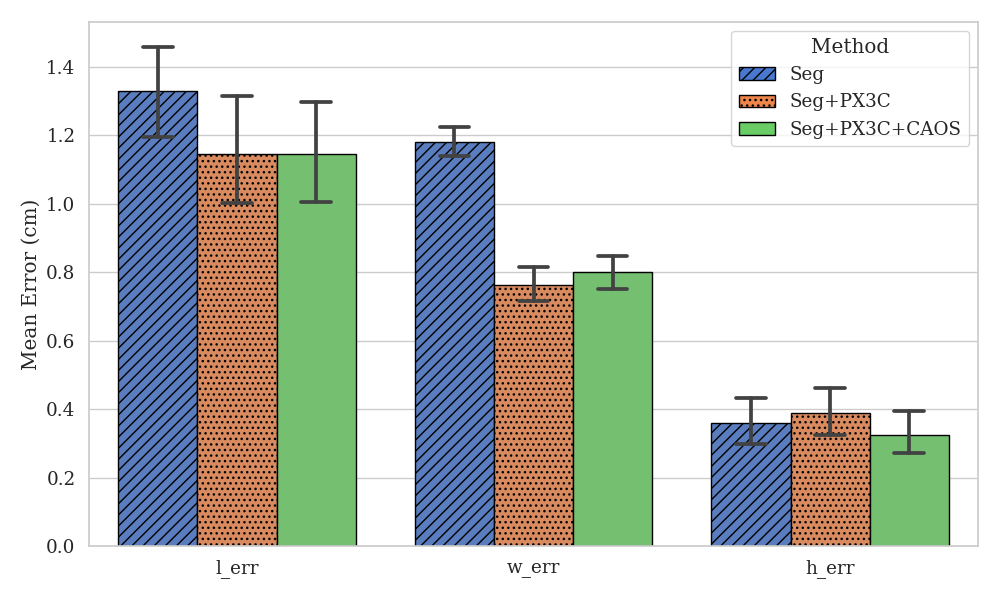
\includegraphics[width=\columnwidth]{figures/fig7.png}
\caption{Comparison of dimension estimation errors before and after PX3C and CAOS. Error bars indicate 95\% confidence intervals.}
\label{fig:estimation}
\end{figure}

\subsection{3D Modeling Accuracy}
To evaluate PX3C and CAOS, dimension and pose estimation errors were computed on OBBData-test. Dimension error was defined as the absolute error in length, width, and height. Pose error included centroid localization error and yaw error in the X--Y plane. Fig.~\ref{fig:estimation} compares dimension estimation before and after PX3C and CAOS, with error bars indicating 95\% confidence intervals.

\begin{figure}[!t]
\centering
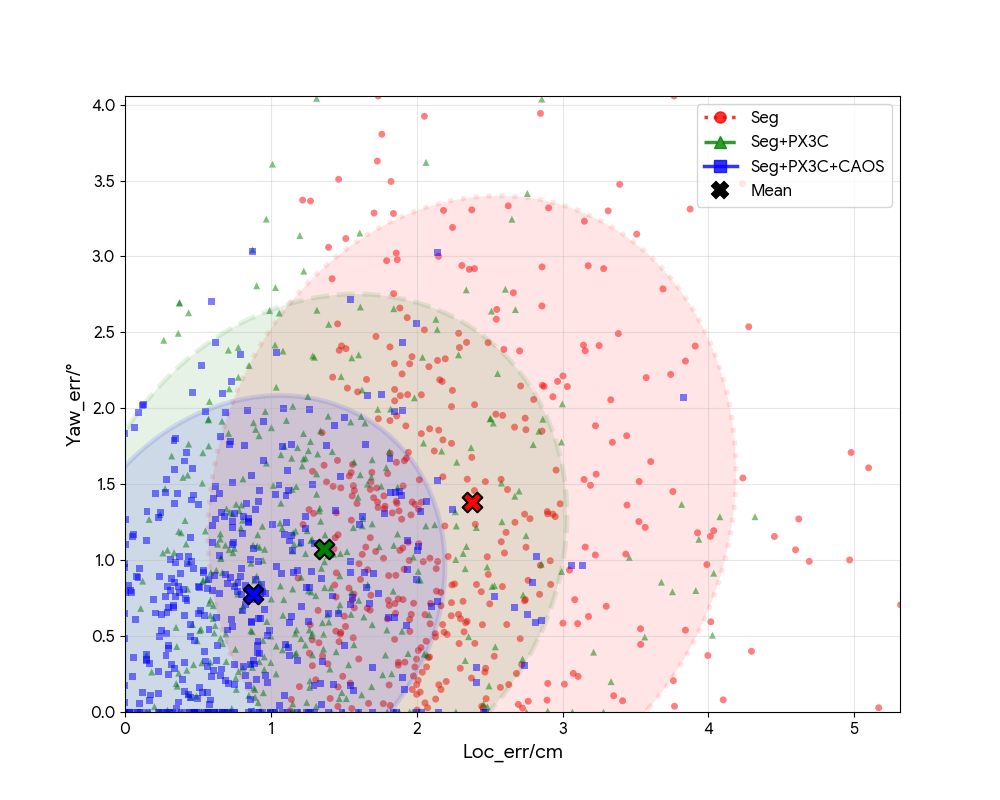
\includegraphics[width=\columnwidth]{figures/fig8.png}
\caption{Localization and yaw error distributions for different modeling stages. Ellipses represent 95\% confidence regions.}
\label{fig:disturbance}
\end{figure}

Compared with segmentation-only modeling, PX3C reduces the width estimation error by 35.5\%. The combined PX3C+CAOS pipeline further stabilizes the estimates. The length estimation error decreases by approximately 13.8\%, and the height estimation error reaches its minimum value of 0.33$\mathrm{cm}$ when both modules are applied. The overall downward shift of the confidence intervals indicates consistent improvement.

The pose-error distributions are shown in Fig.~\ref{fig:disturbance}. Each scatter point corresponds to one sample, and the ellipses denote 95\% confidence regions. Localization error decreases from 2.38$\mathrm{cm}$ using segmentation-only modeling to 1.36$\mathrm{cm}$ with PX3C and to 0.88$\mathrm{cm}$ with CAOS. Yaw error decreases from $1.38^{\circ}$ to $0.78^{\circ}$. These results confirm that PX3C suppresses geometric outliers and CAOS reduces temporal fluctuations.

\begin{figure*}[!t]
\centering
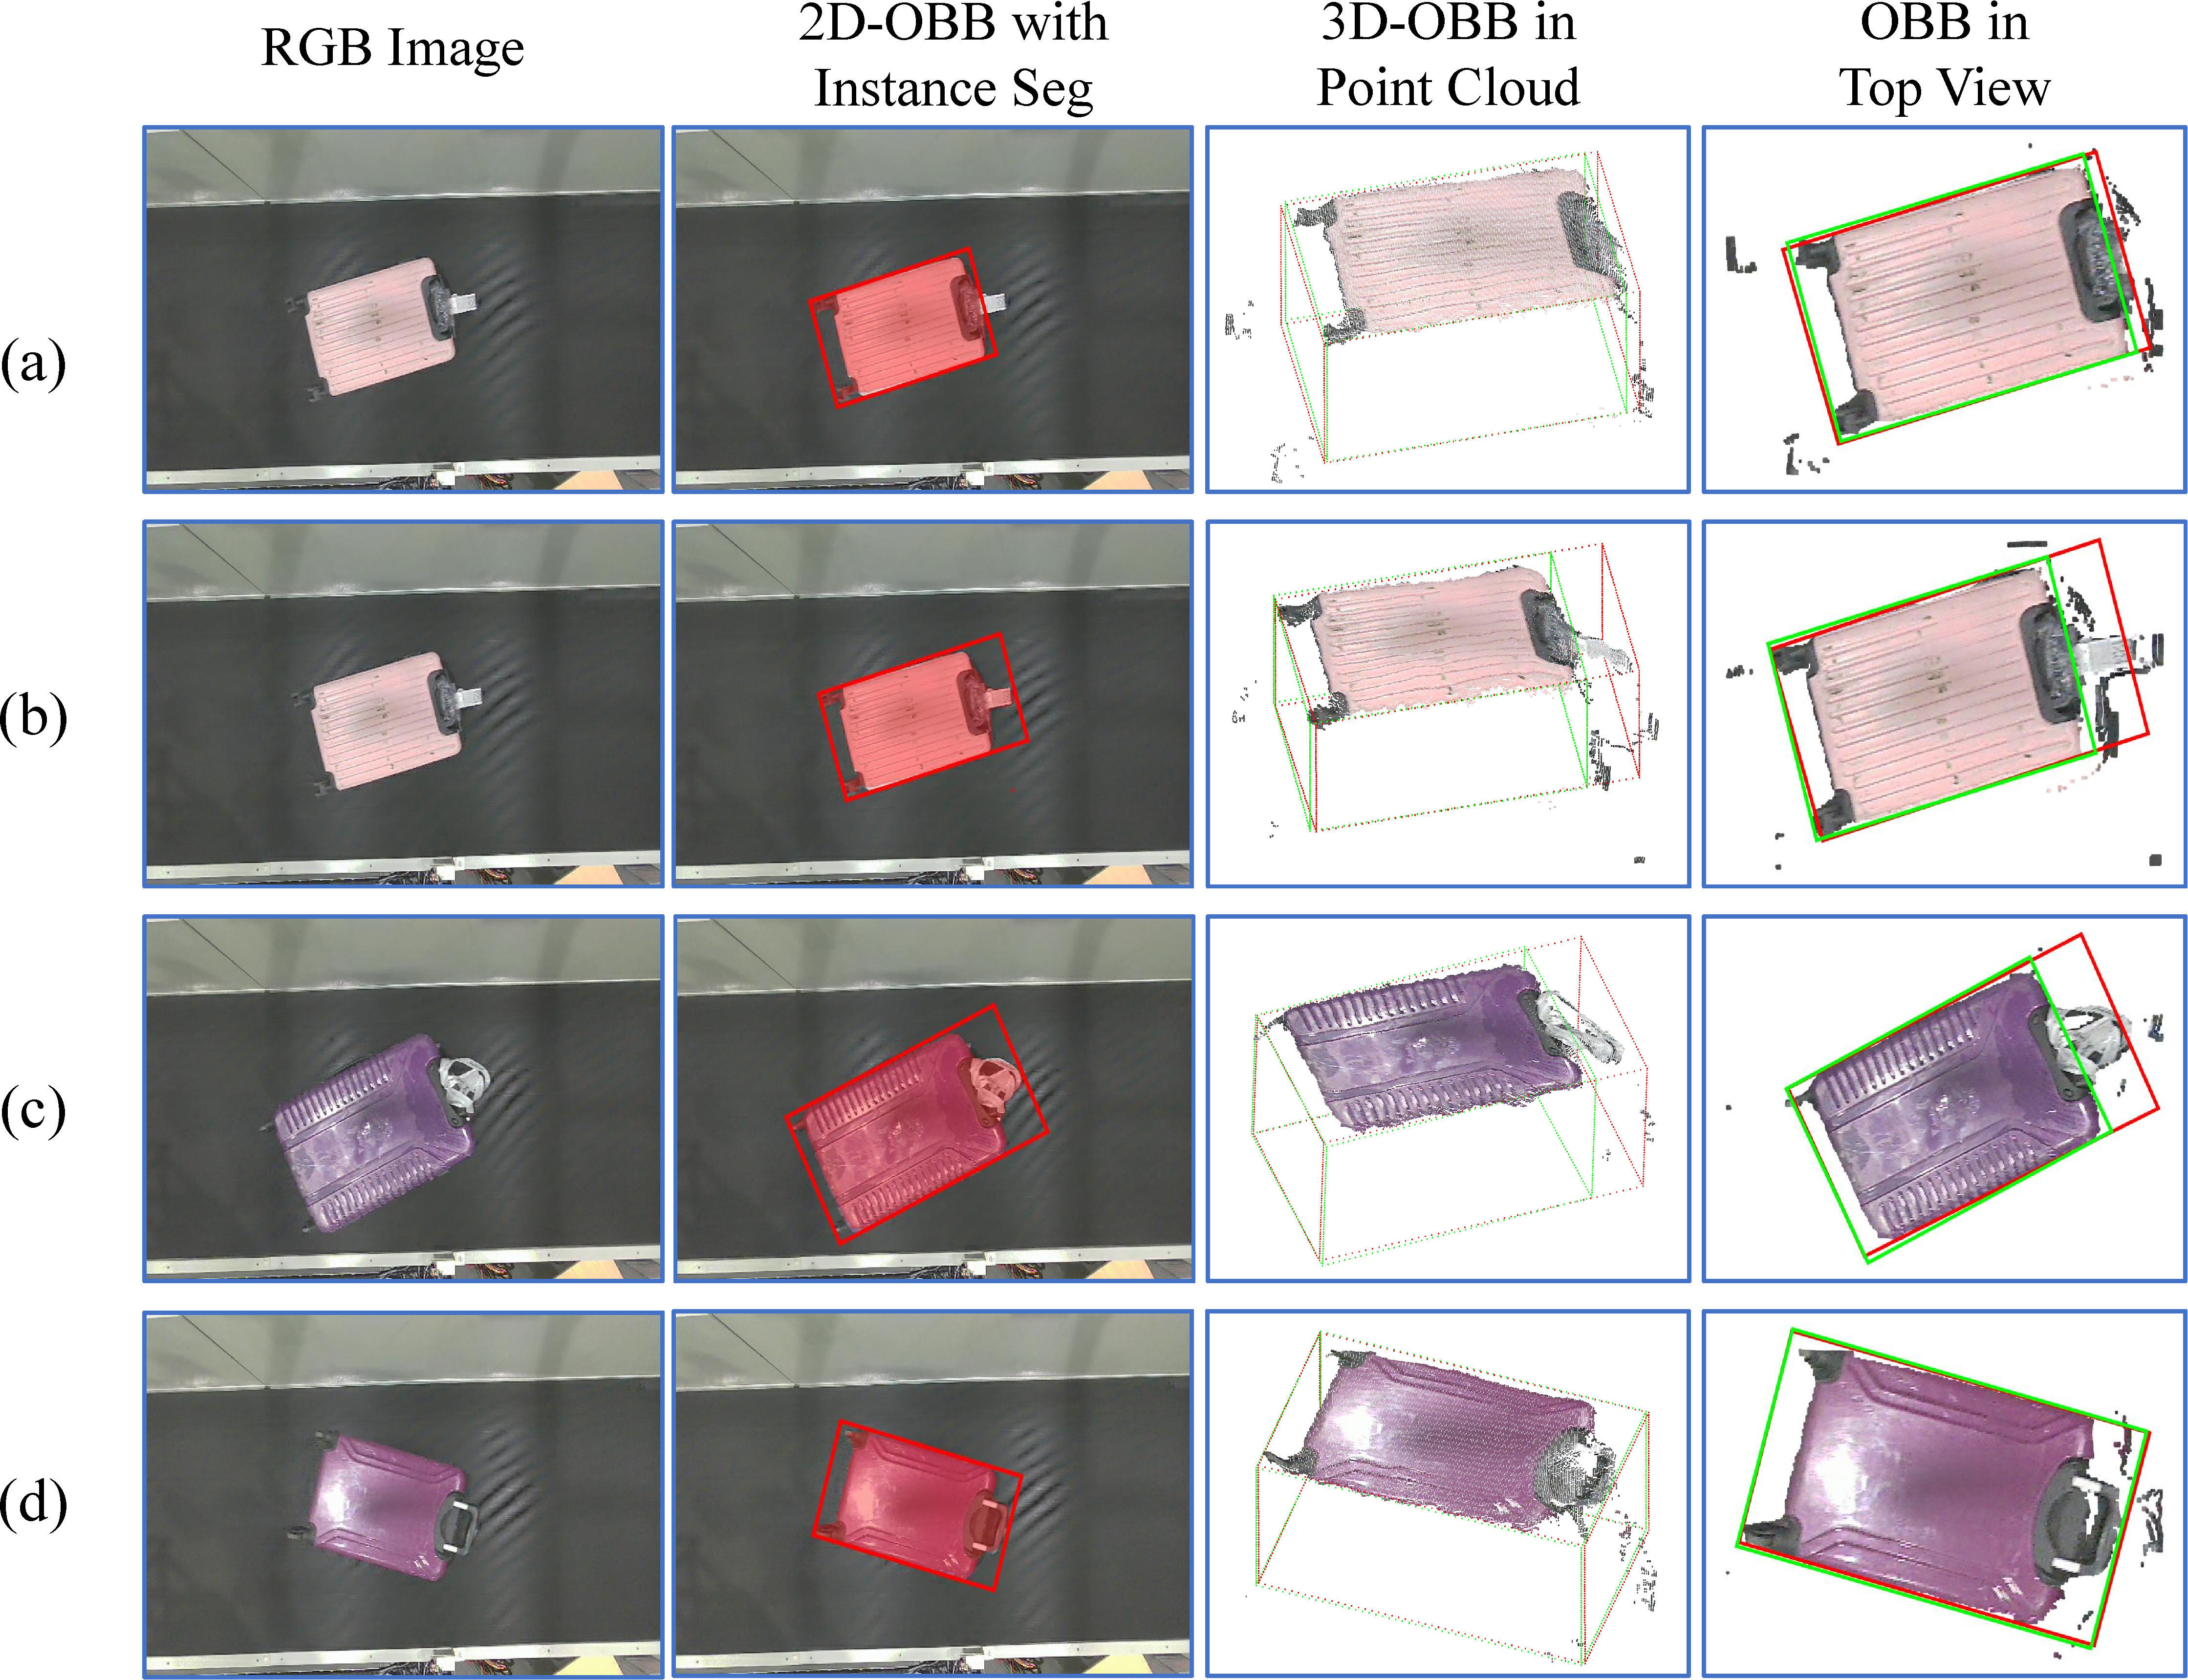
\includegraphics[width=\textwidth]{figures/fig7.pdf}
\caption{Qualitative OBB comparison before and after PX3C filtering.}
\label{fig:represent}
\end{figure*}

Representative qualitative OBB comparisons are shown in Fig.~\ref{fig:represent}. Red boxes denote OBBs derived directly from segmentation, while green boxes denote refined OBBs after PX3C filtering. Flexible tags and ribbons are removed effectively, while rigid components such as handles and wheels are preserved. Temporal stabilization results are shown in Fig.~\ref{fig:temporal}, where CAOS reduces abrupt OBB fluctuations across consecutive frames caused by lighting variation, occlusion, and motion blur.

\begin{figure}[!t]
\centering
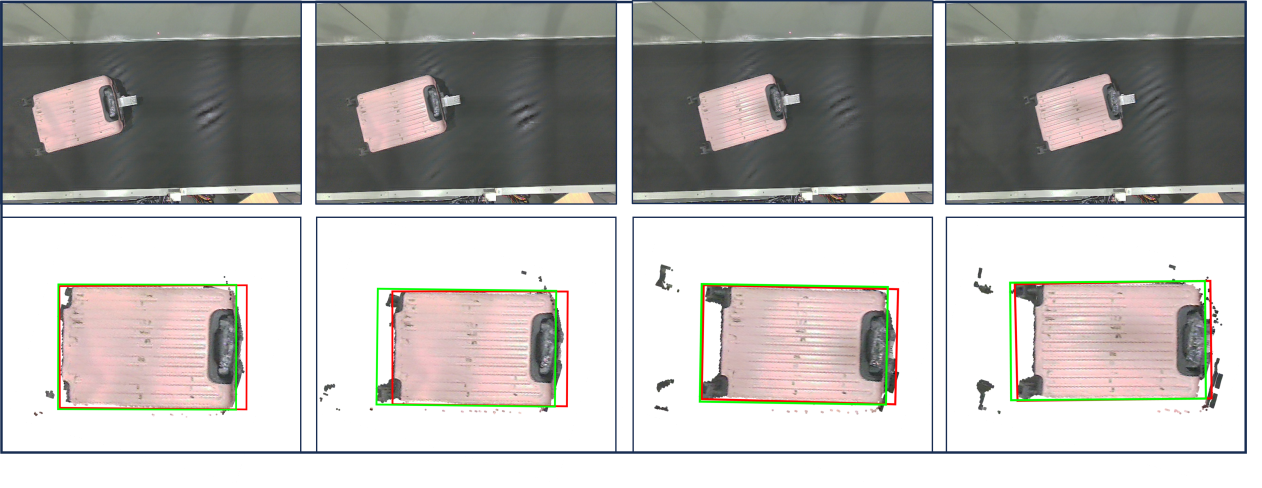
\includegraphics[width=\columnwidth]{figures/fig10.png}
\caption{OBB predictions across consecutive frames with CAOS stabilization.}
\label{fig:temporal}
\end{figure}



\subsection{System-Level Grasping Performance}
Two metrics were used to evaluate system-level performance. General Success Rate (GSR) measures whether the robot successfully lifts the target without dropping it. Precision Success Rate (PSR) requires both a position error below 2$\mathrm{cm}$ and a yaw error below $5^{\circ}$. PSR was computed only for suitcases because they have well-defined geometric references. In multi-object scenarios, the highest object along the Z-axis was selected as the grasping target.

A total of 500 grasping trials were conducted according to the airport baggage distribution, including 470 suitcases, 25 backpacks, and 5 irregular objects. The snapshots are shown in Fig. \ref{fig:snapshot}. An ablation study was performed by incrementally integrating MSAM-Net, PX3C+CAOS, DKF+two-stage planning, and active state regulation. The results are summarized in Table~\ref{tab:ablation}.

\begin{figure*}[!t]
\centering
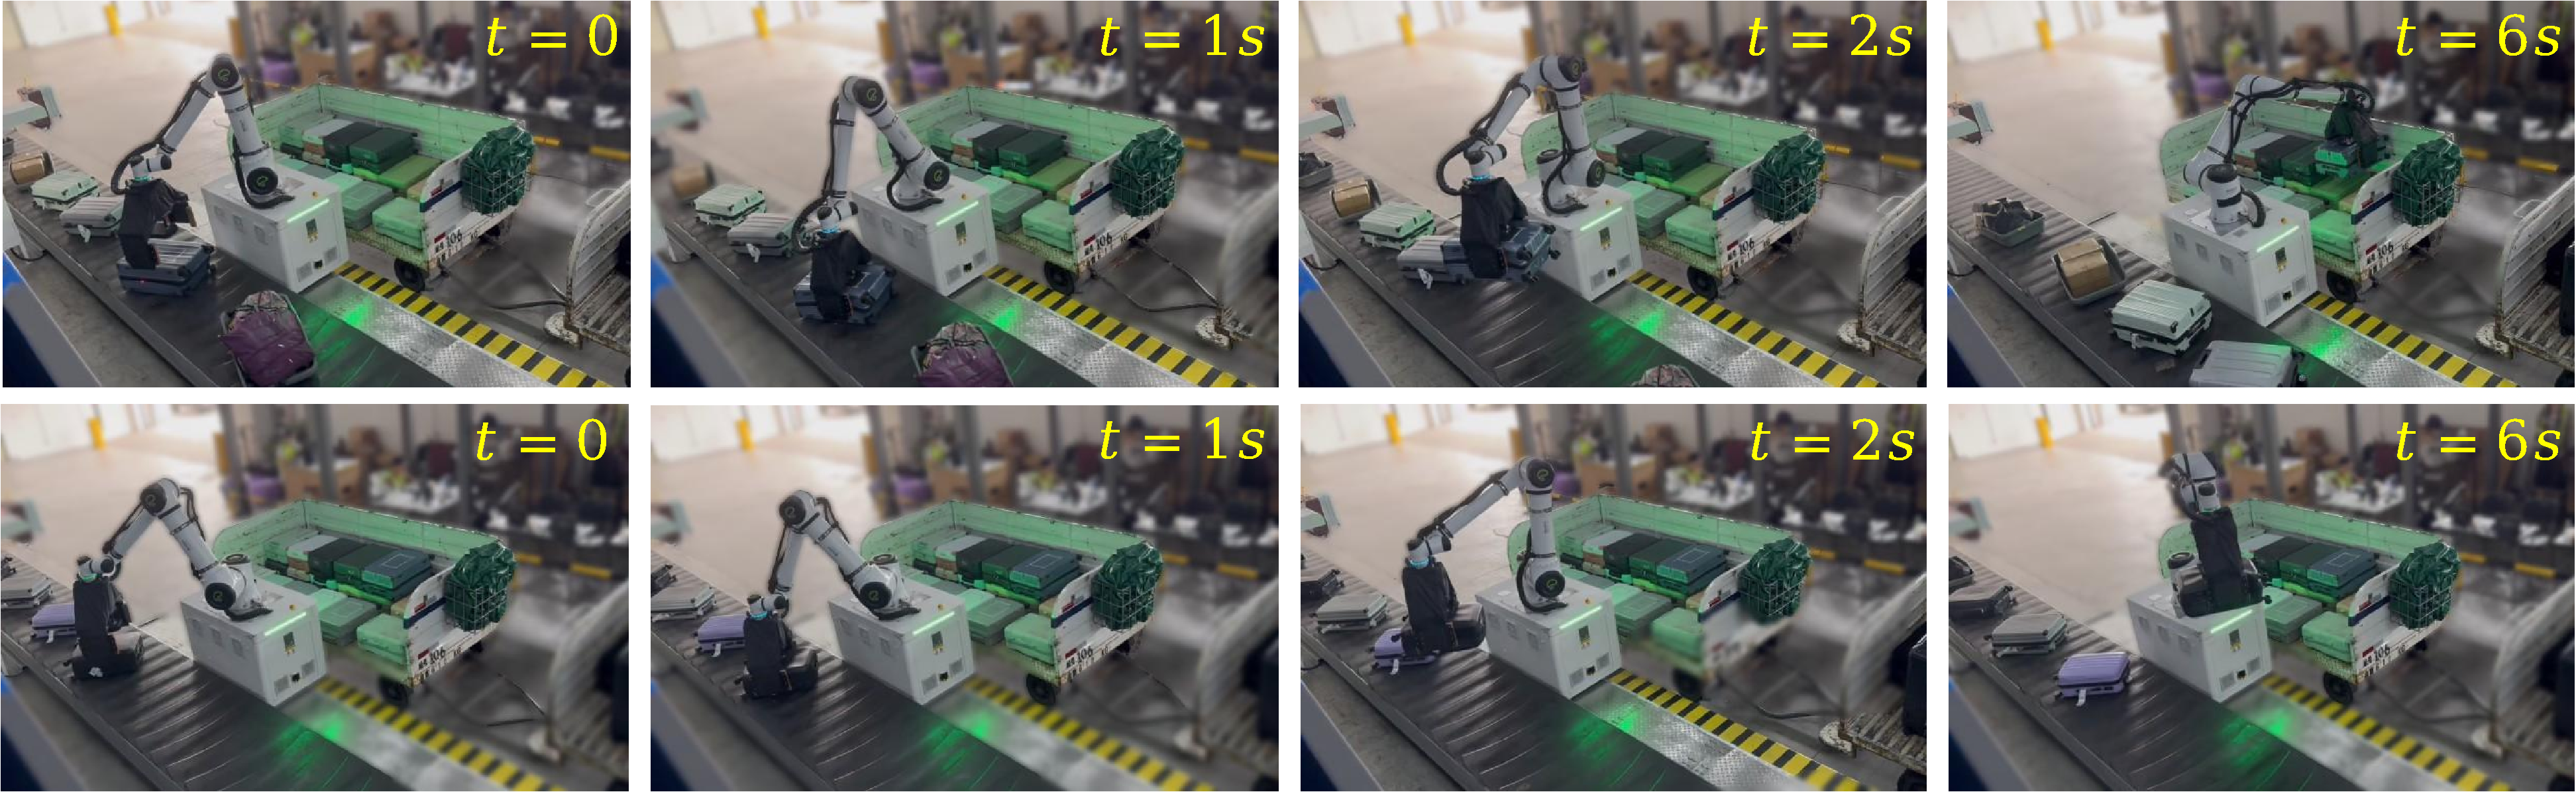
\includegraphics[width=\textwidth]{figures/fig8.pdf}
\caption{Snapshots of the dynamic grasping experiment. The proposed framework achieves robust dynamic grasping on a real conveyor belt in an industrial environment, overcoming the challenges of high-speed motion, cluttered scenes, and control uncertainty.}
\label{fig:snapshot}
\end{figure*}

\begin{table}[!t]
\centering
\caption{Ablation study of different modules on grasping performance.}
\label{tab:ablation}
\begin{tabular}{lcc}
\toprule
Method & GSR (\%) & PSR (\%) \\
\midrule
Baseline (YOLOv10L + PCL) & 93.6 & 62.1 \\
+ Semantic perception (MSAM-Net) & 95.2 & 69.6 \\
+ Geometric consistency (PX3C + CAOS) & 95.6 & 83.8 \\
+ Predictive motion (DKF + two-stage planning) & 96.4 & 84.9 \\
+ Active state regulation (full system) & 96.4 & 92.7 \\
\bottomrule
\end{tabular}
\end{table}

The GSR increases moderately from 93.6\% to 96.4\%, indicating that even the baseline system can lift many objects. In contrast, PSR increases substantially from 62.1\% to 92.7\%. This difference reflects the distinct meanings of the two metrics. GSR primarily measures grasp feasibility, whereas PSR evaluates geometric precision under strict position and orientation constraints. The baseline system can often lift baggage despite moderate pose errors, but inaccurate localization and unstable OBB estimation significantly degrade precise placement. The large PSR improvement demonstrates that the proposed geometric refinement and predictive control modules primarily improve pose accuracy and downstream placement reliability, which are crucial for high-density baggage loading.